\subsection{Adding an environment}
\label{sec:step5_environment}
In this step we will add an environment in which the agents exist and through which they interact with each other. This is a fundamentally different approach to agent interaction but is as valid as the approach in the previous steps. 

In ABS agents are often situated within a discrete 2D environment \cite{epstein_growing_1996} which is simply a finite $N x M$ grid with either a Moore or von Neumann neighbourhood (Figure \ref{fig:abs_neighbourhoods}). Agents are either static or can move freely around with cells allowing either single or multiple occupants.

We can directly map the SIR model to a discrete 2D environment by placing the agents on a corresponding 2D grid with an unrestricted neighbourhood. The behaviour of the agents is the same but they select their interactions directly from the environment. Also instead of feeding back the states of all agents as inputs, agents now communicate through the environment by revealing their current state to their neighbours by placing it on their cell. Agents can read the states of all their neighbours which tells them if a neighbour is infected or not. For purposes of a more interesting approach, we restrict the neighbourhood to Moore (Figure \ref{fig:moore_neighbourhood}).

\begin{figure}
\begin{center}
	\begin{tabular}{c c}
		\begin{subfigure}[b]{0.2\textwidth}
			\centering
			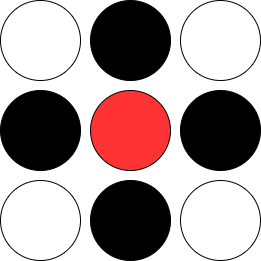
\includegraphics[width=0.5\textwidth, angle=0]{./fig/diagrams/neumann.png}
			\caption{von Neumann}
			\label{fig:neumann_neighbourhood}
		\end{subfigure}
    	&
		\begin{subfigure}[b]{0.2\textwidth}
			\centering
			
\includegraphics[width=0.5\textwidth, angle=0]{./fig/diagrams/moore.png}
			\caption{Moore}
			\label{fig:moore_neighbourhood}
		\end{subfigure}
    \end{tabular}
	\caption{Common neighbourhoods in discrete 2D environments of Agent-Based Simulation.}
	\label{fig:abs_neighbourhoods}
\end{center}
\end{figure}

We also implemented this spatial approach in Java using the well known ABS library RePast \cite{north_complex_2013}, to have a comparison with a state of the art approach and came to the same results as shown in Figure \ref{fig:sir_env}. This supports that our pure functional approach can produce such results as well and compares positively to the state of the art in the ABS field.

\subsubsection{Implementation}
We start by defining our discrete 2D environment for which we use an indexed two dimensional array. In each cell the agents will store their current state, thus we use the \textit{SIRState} as type for our array data:

\begin{HaskellCode}
type Disc2dCoord = (Int, Int)
type SIREnv      = Array Disc2dCoord SIRState
\end{HaskellCode}

Next we redefine our monad stack and agent signal function. We use a StateT transformer on top of our Random Monad from the previous step with \textit{SIREnv} as type for the state. Our agent signal function now has unit input and output type, which indicates that the actions of the agents are only visible through side-effects in the monad stack they are running in.

\begin{HaskellCode}
type SIRMonad g = StateT SIREnv (Rand g)
type SIRAgent g = SF (SIRMonad g) () ()
\end{HaskellCode}

The implementation of a susceptible agent is now a bit different. The agent directly queries the environment for its neighbours and randomly selects one of them. The remaining behaviour is similar:

\begin{HaskellCode}
susceptibleAgent :: RandomGen g => Disc2dCoord -> SIRAgent g
susceptibleAgent coord
    = switch susceptible (const (infectedAgent coord))
  where
    susceptible :: RandomGen g 
      => SF (SIRMonad g) () ((), Event ())
    susceptible = proc _ -> do
      makeContact <- occasionallyM (1 / contactRate) () -< ()
      if not (isEvent makeContact)
        then returnA -< ((), NoEvent)
        else (do
          env <- arrM_ (lift get) -< ()
          let ns = neighbours env coord agentGridSize moore
          s <- drawRandomElemS -< ns
          case s of
            Infected -> do
              infected <- arrM_ 
                (lift $ lift $ randomBoolM infectivity) -< ()
              if infected 
                then (do
                  arrM (put . changeCell coord Infected) -< env
                  returnA -< ((), Event ()))
                else returnA -< ((), NoEvent)
            _        -> returnA -< ((), NoEvent))

neighbours :: SIREnv -> Disc2dCoord -> Disc2dCoord 
           -> [Disc2dCoord] -> [SIRState]
           
moore :: [Disc2dCoord]
moore = [ topLeftDelta,    topDelta,     topRightDelta,
          leftDelta,                     rightDelta,
          bottomLeftDelta, bottomDelta,  bottomRightDelta ]

topLeftDelta :: Disc2dCoord
topLeftDelta      = (-1, -1)
topDelta :: Disc2dCoord
topDelta          = ( 0, -1)
...
\end{HaskellCode}
Querying the neighbourhood is done using the \textit{neighbours} function. It takes the environment, the coordinate for which to query the neighbours for, the dimensions of the 2D grid and the neighbourhood information and returns the data of all neighbours it could find. Note that on the edge of the environment, it could be the case that fewer neighbours than provided in the neighbourhood information will be found due to clipping.

The behaviour of an infected agent is similar to in the previous step, with the difference that upon recovery the infected agent updates its state in the environment from Infected to Recovered.

For running the simulation with MSFs we use the function \textit{embed} which is not provided by BearRiver but by Dunai which has important implications. As already explained in the background Section \ref{sec:back_msf}, Dunai does not know about time in MSFs, which is what BearRiver builds on top of MSFs. Thus, when running our simulation using \textit{embed} we get the \textit{ReaderT} in addition to the other Monad Transformers, which we need to run using \textit{runReaderT}. Note that instead of returning agent states we simply return a list of environments, one for each step. The agent states can then be extracted from each environment.

\begin{HaskellCode}
runSimulation :: RandomGen g => g -> Time -> DTime 
  -> SIREnv -> [(Disc2dCoord, SIRState)] -> [SIREnv]
runSimulation g t dt env as = evalRand esRand g
  where
    steps    = floor (t / dt)
    dts      = replicate steps ()
    -- initial SFs of all agents
    sfs      = map (uncurry sirAgent) as   
    -- running the simulation   
    esReader = embed (stepSimulation sfs) dts 
    esState  = runReaderT esReader dt 
    esRand   = evalStateT esState env     
\end{HaskellCode}

Due to the different approach of returning the SIREnv in every step, we implemented our own MSF:
\begin{HaskellCode}
stepSimulation :: RandomGen g 
  => [SIRAgent g] -> SF (SIRMonad g) () SIREnv
stepSimulation sfs = MSF (\_ -> do
  -- running all SFs with unit input
  res <- mapM (`unMSF` ()) sfs
  -- extracting continuations, ignore output
  let sfs' = fmap snd res
  -- getting environment of current step   
  env <- get
  -- recursive continuation    
  let ct = stepSimulation sfs'  
  return (env, ct))
\end{HaskellCode}

\subsubsection{Results}
We implemented rendering of the environments using the gloss library which allows us to cycle arbitrarily through the steps and inspect the spreading of the disease over time visually as seen in Figure \ref{fig:sir_env}.

\begin{figure}
\begin{center}
	\begin{tabular}{c c}
		\begin{subfigure}[b]{0.2\textwidth}
			\centering
			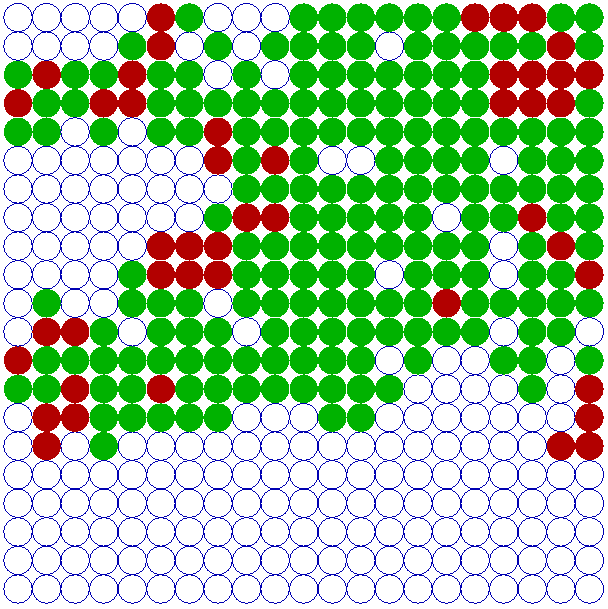
\includegraphics[width=1\textwidth, angle=0]{./fig/step5_environment/SIR_environment_30x30agents_t100_01dt.png}
			\caption{$t = 100$}
			\label{fig:sir_env_t100}
		\end{subfigure}
    	
    	&
  
		\begin{subfigure}[b]{0.23\textwidth}
			\centering
			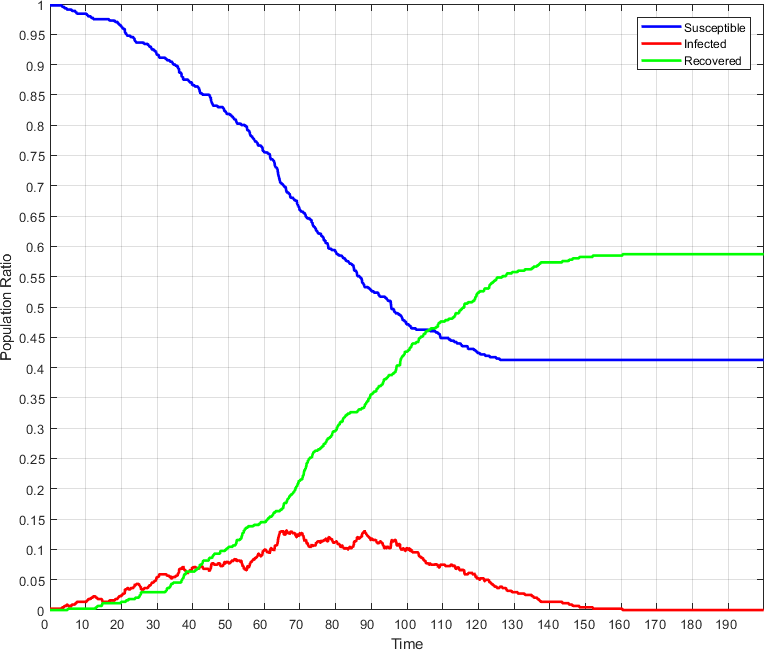
\includegraphics[width=1\textwidth, angle=0]{./fig/step5_environment/SIR_dynamics_30x30agents_300t_01dt.png}
			\caption{Dynamics over time}
			\label{fig:sir_dynamics_30x30agents_300t_01dt}
		\end{subfigure}
	\end{tabular}
	
	\caption{Simulating the agent-based SIR model on a 21x21 2D grid with Moore neighbourhood (Figure \ref{fig:moore_neighbourhood}), a single infected agent at the center and same SIR parameters as in Figure \ref{fig:sir_sd_dynamics}. Simulation run until $t = 200$ with fixed $\Delta t = 0.1$. Last infected agent recovers shortly after $t = 160$. The susceptible agents are rendered as blue hollow circles for better contrast.}
	\label{fig:sir_env}
\end{center}
\end{figure}

Note that the dynamics of the spatial SIR simulation which are seen in Figure \ref{fig:sir_dynamics_30x30agents_300t_01dt} look quite different from the reference dynamics of Figure \ref{fig:sir_sd_dynamics}. This is due to a much more restricted neighbourhood which results in far fewer infected agents at a time and a lower number of recovered agents at the end of the epidemic, meaning that fewer agents got infected overall.

\subsubsection{Discussion}
At first the environment approach might seem a bit overcomplicated and one might ask what we have gained by using an unrestricted neighbourhood where all agents can contact all others. The real advantage is that we can introduce arbitrary restrictions on the neighbourhood as shown with the Moore neighbourhood.

Of course an environment is not restricted to be a discrete 2D grid and can be anything from a continuous N-dimensional space to a complex network - one only needs to change the type of the StateT monad and provide corresponding neighbourhood querying functions. The ability to place the heterogeneous agents in a generic environment is also the fundamental advantage of an agent-based over other simulation approaches and allows us to simulate much more realistic scenarios.